\documentclass[a4paper,14pt]{article}

\usepackage{comment} % Para comentar várias linhas ao mesmo tempo

%matemática
\usepackage{amsmath}
\usepackage{amssymb}

%diagramação
\usepackage{extsizes}
\everymath{\displaystyle}
\usepackage{geometry}
\usepackage{fancyhdr}
\usepackage{multicol}
\usepackage{graphicx}
\usepackage[brazil]{babel}
\usepackage[shortlabels]{enumitem}
\usepackage{cancel}
\usepackage{textcomp}
\usepackage{tcolorbox}

%tabelas
\usepackage{array} % Para melhor formatação de tabelas
\usepackage{longtable}
\usepackage{booktabs}  % Para linhas horizontais mais bonitas
\usepackage{float}   % Para usar o modificador [H]
\usepackage{caption} % Para usar legendas em tabelas
\usepackage{wrapfig} % Para usar tabelas e figuras flutuantes
\usepackage{xcolor} % Para cores do fundo de tabelas
\usepackage{colortbl} % Para cores do fundo de tabelas
\usepackage{upgreek} % Para inserir caracteres gregos

%tikzpicture
\begin{comment}
	\usepackage{tikz}
	\usepackage{scalerel}
	\usepackage{pict2e}
	\usepackage{tkz-euclide}
	\usetikzlibrary{calc}
	\usetikzlibrary{patterns,arrows.meta}
	\usetikzlibrary{shadows}
	\usetikzlibrary{external}
\end{comment}


%pgfplots
\usepackage{pgfplots}
\pgfplotsset{compat=newest}
\usepgfplotslibrary{statistics}
\usepgfplotslibrary{fillbetween}

%colours
\usepackage{xcolor}



\columnsep=2cm
\hoffset=0cm
\textwidth=8cm
\setlength{\columnseprule}{.1pt}
\setlength{\columnsep}{2cm}
\renewcommand{\headrulewidth}{0pt}
\geometry{top=1in, bottom=1in, left=0.7in, right=0.5in}

\pagestyle{fancy}
\fancyhf{}
\fancyfoot[C]{\thepage}

\begin{document}
	
	\noindent\textbf{6FMA148 - Matemática} 
	
	\begin{center}Aproximações (Versão estudante)
	\end{center}
	
	\noindent\textbf{Nome:} \underline{\hspace{10cm}}
	\noindent\textbf{Data:} \underline{\hspace{4cm}}
	
	%\section*{Questões de Matemática}
	
	\begin{multicols}{2}
	    \noindent Para aproximar um número, devemos compará-lo com o múltiplo de dez mais próximo. \\
	    Exemplos: 
	    \textbf{a)} 73 \\
	    O múltiplo da potência de dez mais próximo é $70 = 7 \cdot 10$, ou seja, a aproximação de 70 é $7 \cdot 10^1$. \\
	    \textbf{b)} 192 \\
	    O múltiplo da potencia de dez mais próximo é $200 = 2 \cdot 10^2$, ou seja, a aproximação de 200 é $2 \cdot 10^2$. \\
	    \\
	    Ordem de grandeza é a potência de dez inteira mais próxima de um valor. \\
	    Exemplos: \\
	    \textbf{a)} 400 \\
	    Sabemos que $400 = 4 \cdot 10^2$. Logo, a ordem de grandeza é $10^2$. \\
	    \textbf{b)} $92 000 \cdot 10^7$ \\
	    Sabemos que $92 000 \cdot 10^7 = 9,2 \cdot 10^4 \cdot 10^7 = 9,2 \cdot 10^11$, e como 9,2 é maior que 5,5, a ordem de grandeza de $92 000 \cdot 10^7$ é $10^{12}$. \\
		\noindent\textsubscript{--------------------------------------------------------------------------}
		\begin{enumerate} 
			\item Faça a aproximação dos números a seguir utilizando um múltiplo de potência de dez:
			\begin{enumerate}[a)]
				\item 6 \\\\\\
				\item 12 \\
				\item 34 \\\\\\
				\item 94 \\\\\\
				\item 146 \\\\\\
				\item 439 \\\\\\
				\item 791 \\\\\\
				\item 1 456 \\\\\\
				\item 3 970 \\\\\\
				\item 2 504 \newpage
			\end{enumerate}
			\item Localize na reta as potências de dez mais próximas aos valores dados:
			\begin{enumerate}[a)]
				\item 74 \\
				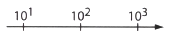
\includegraphics[width=1\linewidth]{6FMA148_imagens/imagem1} \\\\\\\\\\\\\\\\\\
				\item 930 \\
				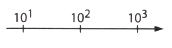
\includegraphics[width=1\linewidth]{6FMA148_imagens/imagem2} \\\\\\\\\\\\\\\\\\
				\item 140 \\
				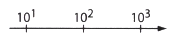
\includegraphics[width=1\linewidth]{6FMA148_imagens/imagem3} \\\\\\\\\\\\\\
				\item 1 024 \\
				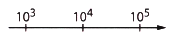
\includegraphics[width=1\linewidth]{6FMA148_imagens/imagem4} \\\\\\\\\\\\\\\\\\
				\item 40 601 \\
				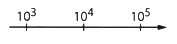
\includegraphics[width=1\linewidth]{6FMA148_imagens/imagem5} \\\\\\\\\\\\\\\\\\
				\item 204 618 \\
				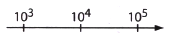
\includegraphics[width=1\linewidth]{6FMA148_imagens/imagem6} \newpage
			\end{enumerate}
			\item Determine a ordem de grandeza dos seguintes números:
			\begin{enumerate}[a)]
				\item $5,1 \cdot 10^{24}$ \\\\\\\\
				\item $35,8 \cdot 10^{135}$ \\\\\\\\
				\item $467,8 \cdot 10^{67}$ \\\\\\\\
				\item $37 \cdot 10^{1064}$ \\\\\\\\
				\item $600 \cdot 10^7$ \\\\\\\\
				\item $49 \cdot 10^{297}$ \\\\\\\\
			\end{enumerate}
			\item Mariana decide ir à feira comprar 5 maçãs, 3 peras, 6 laranjas e 1 melão. Ela sabe que os preços por unidade da maçã, da pera, da laranja e do melão são, respectivamente, R\$ 1,75, R\$ 3,25, R\$ 2,02 e R\$ 15,87. Qual será o gasto aproximado de Mariana nessa compra? Ela conseguirá pagar sua compra se levar apenas duas notas de 20 reais? Justifique. \\\\\\\\\\\\\\\\\\\\\\\\
			\textbf{Desafio olímpico} \\\\
			Para $\frac{24 \cdot 0,2 \cdot 40,12}{99}$, qual das alternativas apresenta o resultado mais próximo?
			\begin{enumerate}[a)]
				\item 0,02
				\item 100
				\item 0,1
				\item 10
				\item 2 \newpage
			\end{enumerate}
			%9 a 12
			\item Localize na reta as potências de dez mais próximas aos valores dados:
			\begin{enumerate}[a)]
				\item 26 \\
				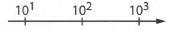
\includegraphics[width=1\linewidth]{6FMA148_imagens/imagem7}
				\item 1 346 \\
				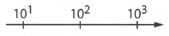
\includegraphics[width=1\linewidth]{6FMA148_imagens/imagem8}
				\item 761 \\
				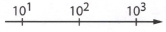
\includegraphics[width=1\linewidth]{6FMA148_imagens/imagem9}
				\item 10 542 \\
				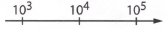
\includegraphics[width=1\linewidth]{6FMA148_imagens/imagem10}
			\end{enumerate}
			\item Aproxime os números abaixo para os múltiplos das potências de 10 mais próximos:
			\begin{enumerate}[a)]
				\item 13 \\\\
				\item 39 \\\\
				\item 43 \\\\
				\item 87 \\\\
				\item 126 \\\\
				\item 391 \\\\
				\item 681 \\\\
				\item 973 \\\\
				\item 1 379 \\\\
				\item 97 016 \\\\
				\item 326 789 \\\\
				\item 761 432 150 \\\\
			\end{enumerate}
			\item Qual é a ordem de grandeza dos números abaixo:
			\begin{enumerate}[a)]
				\item $4,9 \cdot 10^{73}$ \\\\
				\item $46,98 \cdot 10^{342}$ \\\\
				\item $21,47 \cdot 10^{137}$ \\\\
				\item $932 \cdot 10^{210}$ \\\\
				\item $4 000 \cdot 10^9$ \\\\
				\item $215,12 \cdot 10^{349}$ \\\\
				\item $0,0798 \cdot 10^{46}$ \\\\
				\item $0,0071 \cdot 10^{600}$ \\\\
				\item $346 \cdot 10^{2009}$ \\\\
				\item $74,15 \cdot 10^{705}$ \\\\
			\end{enumerate}
			\item Paulo está fazendo uma reforma em sua casa e decidiu colocar azulejos em seu banheiro. Em uma parede de 3,96 metros por 2,83 metros, ele irá colocar um azulejo quadrado de 10 cm de lado. Sabendo que estes azulejos são vendidos em caixas com 100 unidades, quantas destas caixas Paulo deve comprar? \\\\\\\\\\\\\\\\\\\\\\\\
		\end{enumerate}
		 $~$ \\ $~$ \\ $~$ \\ $~$ \\ $~$ \\ $~$ \\ $~$ \\ $~$ \\ $~$ \\ $~$ \\ $~$ \\ $~$ \\ $~$ \\ $~$ \\ $~$ \\ $~$ \\ $~$ \\ $~$ \\ $~$ \\ $~$ \\ $~$ \\ $~$ \\ $~$ \\ $~$ \\ $~$ \\ $~$ \\ $~$ \\ $~$ \\ $~$ \\ $~$ \\ $~$ \\ $~$ \\ $~$ \\ $~$ \\ $~$ \\ $~$ \\ $~$ \\ $~$ \\ $~$ \\ $~$ \\ $~$ \\ $~$ \\ $~$ \\ $~$ \\
	\end{multicols}
\end{document}